\chapter{Penetrationstest}
\label{chap:k4}

\section{Überblick}

Sicherheit ist eines der größten Probleme von Informationssystemen. Penetrationstests sind eine wichtige Sicherheitsbewertungsmethode und eine effektive Methode zur Beurteilung der Sicherheitslage eines bestimmten Informationssystems. In vielen Webanwendungen verbergen sich verschiedene Sicherheitslücken, die dem Betreiber nicht wahrnehmbar sind. Mittels dieser Sicherheitslücken entsteht ein großes Sicherheitsrisiko, weil ein Angreifer unter Umständen eine Lücke findet, die ihm unautorisierten Zugriff auf das System gewährt. Um dieses Risiko zu vermindern, werden Penetrationstests durchgeführt.

Der Umfang eines Penetrationstests kann von einzelnen Anwendungen bis zu unternehmensweiten Angriffen stark variieren. Ein Penetrationstest, der häufig mit einem Schwachstellenscan oder einer Schwachstellenanalyse verwechselt wird, versucht nicht nur, Schwachstellen zu finden, sondern sie auch in vollem Umfang auszunutzen. Dies bedeutet, dass ein Penetrationstester zwar mit der Suche nach einer Schwachstelle beauftragt werden kann, dass er jedoch alle entdeckten Schwachstellen verwendet und weiterhin ein System angreift, um mögliche zusätzliche Schwachstellen zu ermitteln\cite{northcutt2006}.


\section{Definitionen}

Bei einem Penetrationstest handelt es sich um die Sicherheit der IT-Systeme durch Bedrohungen von Angreifern inwiefern gefährdet ist bzw. ob die IT-Sicherheit durch die Sicherheitsmaßnahmen gewährleistet ist. Es werden unterschiedliche Methoden bei einem Penetrationstest verwendet, die auch von einem Angreifer durchgeführt würde. \cite[5--6]{pt03bsi}. Ein Penetrationstest für Webanwendungen konzentriert sich nur auf die Bewertung der Sicherheit einer Webanwendung. Der Prozess beinhaltet eine aktive Analyse der Anwendung auf Schwachstellen, technische Fehler oder Verwundbarkeit. Alle gefundenen Sicherheitsprobleme werden dem Systembetreiber zusammen mit einer Bewertung der Auswirkungen und häufig mit einem Vorschlag zur Milderung oder einer technischen Lösung vorgelegt\cite[46]{meucci2008owasp}.

In Bezug auf Penetrationstests gibt es eine Vielzahl von Definitionen. Nach dem von Bacudio\cite{bacudio2011overview} und Ke\cite{ke2009using} definierten Penetrationstest handelt es sich um eine Reihe von Aktivitäten zur Ermittlung und Ausnutzung von Sicherheitsschwächen. Es ist ein Sicherheitstest, bei dem versucht wird, Sicherheitsmerkmale eines Systems zu umgehen\cite{wack2003guideline}. Osborne definiert einen Penetrationstest als einen Test, mit dem sichergestellt wird, dass Gateways, Firewalls und Systeme entsprechend konzipiert und konfiguriert sind, um vor unberechtigtem Zugriff oder dem Versuch zu schützen, Dienste zu stören\cite{osborne2006cheat}.

\section{Ziele der Penetrationstests}

Da es kein System gibt, das weder jetzt noch in der Zukunft zu \%100 sicher ist, besteht eines der Hauptziele der Penetrationstests darin, zu prüfen, wie sicher ein System ist, dh wie unsicher es aus der Sicht eines Hackers ist. Um detaillierter zu erklären, werden Penetrationstests verwendet, um Lücken in der Sicherheitslage zu identifizieren, Exploits zu verwenden, um in das Zielnetzwerk zu gelangen, und dann Zugriff auf vertrauliche Daten zu erhalten\cite{yeo2013using}.

National Institute of Standards and Technology legt nahe, dass Penetrationstests auch zur Bestimmung von Folgendem nützlich sein können\cite{scarfone2008technical}: 

\begin{itemize}
	\item Wie gut das System reale Angriffsmuster toleriert.{\color{red}(How well the system tolerates real world attack patterns.)}
	\item Die wahrscheinliche Komplexität, die ein Angreifer benötigt, um das System erfolgreich zu beeinträchtigen.
	\item Zusätzliche Gegenmaßnahmen, die Bedrohungen gegen das System abschwächen könnten.
	\item Fähigkeit der Verteidiger, Angriffe zu erkennen und angemessen zu reagieren.
\end{itemize}

\section{Grundlegendes Konzept}

Penetrationstests können auf verschiedene Arten durchgeführt werden. Der häufigste Unterschied ist das Wissen über die Implementierungsdetails der getesteten Systeme, die dem Tester zur Verfügung gestellt wurden. Die weithin akzeptierten Ansätze sind Black-Box-, White-Box- und Gray-Box-Tests.

\begin{figure}[h]
	\centering
	
\includegraphics[width=\textwidth]{blackwhitegray.jpg}
	\caption{Die akzeptierte Ansätze\cite{bwgtesting16}}
\end{figure}

\subsection{Black-Box}

Black-Box-Tests beziehen sich auf das Testen eines Systems ohne spezifische Kenntnisse der internen Abläufe des Systems, keinen Zugriff auf den Quellcode und keine Kenntnisse der Architektur\cite{bwgwebtesting07}. Dem Tester wird nichts über das Netzwerk oder die Umgebung des Ziels mitgeteilt\cite{tiller2004ethical}. Wenn es sich um einen Black-Box-Test handelt, kann dem Tester eine Webseite oder IP-Adresse zugewiesen werden, und er soll die Website so knacken, als wäre er ein böswilliger Hacker von außen\cite{whitaker2005penetration}. Aufgrund des Mangels an internem Anwendungswissen kann das Aufdecken von Fehlern und / oder Schwachstellen jedoch erheblich länger dauern. Black-Box-Tests müssen gegen laufende Instanzen von Anwendungen ausgeführt werden. Daher ist Black-Box-Tests normalerweise auf dynamische Analysen wie das Ausführen von automatisierten Scan-Tools und manuelle Penetrationstests beschränkt\cite{bwgwebtesting07}. In Black-Box-Sicherheitstests können Hacker verschiedener Fertigkeitsstufen wie z. B. Skript-Kiddies, Mid-Level-Hacker oder Elite-Hacker\cite{bwgprole18}.

\subsection{White-Box}

Die White-Box-Tests werden auch als "interne Tests" bezeichnet. Bei diesem Ansatz simulieren Tester einen Angriff als eine Person, die über vollständige Kenntnisse der zu testenden Infrastruktur verfügt, häufig Betriebssystemdetails, IP-Adressschema und Netzwerklayouts, Quellcode und möglicherweise sogar einige Kennwörter\cite{ali2011pt}. Durch den vollständigen Zugriff auf diese Informationen können Fehler und Schwachstellen schneller entdeckt werden als mit der Test- und Fehlermethode des Black-Box-Tests. Darüber hinaus können Sie sicher sein, eine umfassendere Testabdeckung zu erhalten, indem Sie genau wissen, was Sie testen müssen. Aufgrund der Komplexität der Architekturen und des Umfangs des Quellcodes führt das White-Box-Testen jedoch zu Herausforderungen, wie die Test- und Analysebemühungen am besten ausgerichtet werden können. Zur Unterstützung von White-Box-Tests sind normalerweise Fachwissen und Tools erforderlich, z. B. Pentesting-Tool, Debugger und Quellcode-Analysatoren\cite{bwgwebtesting07}.

\section{Kriterien für Penetrationstests}

Bei einem Penetrationstest gibt es eine Vielzahl von verschiedenen Zielsetzungen, die vor dem Test festgelegt
werden müssen. Somit kann bei einem Penetrationstest ein realistischer Angriff simuliert werden, aber auch
ein Angriff von Insidern, die das Firmennetzwerk von ihrer täglichen Arbeit sehr gut kennen. Hierfür gibt es
verschiedene Kriterien, die vor einem Test berücksichtigt werden müssen. Im Nachfolgenden werden diese
Kriterien nach der Studie für Penetrationstests des BSI\cite{pt03bsi} beschrieben.

\subsection{Informationsbasis}

Bei der Informationsbasis muss entschieden werden, wie viel Information der Tester über das anzugreifende
Ziel erhalten soll. Hier unterscheidet man zwischen Black-Box- und White-Box-Test. Bei einem Black-Box-Test bekommt der Tester nur sehr wenig bis zu keiner Information über das Angriffsziel. Dieser Test simuliert einen realistischen Angriff, da der Tester sich erst mit dem zu testenden System auseinandersetzen muss, um Details zu recherchieren, wie zum Beispiel welche Dienste mit welchen Versionsnummern
dort laufen. Dies ist für den Tester sehr aufwendig und zeitintensiv. Im Gegensatz zu einem Black-Box-Test bekommt der Tester bei einem White-Box-Test mehr Informationen
zu dem Angriffsziel. Ein solcher Test soll zeigen, wie weit ein Insider mit sehr viel Wissen über die IT-Infrastruktur
des Unternehmens in das Ziel eindringen kann. Hierfür bekommt der Tester den vollen Umfang
an Informationen wie IP-Adressen, verwendete Netzwerkprotokolle und den Source Code von Anwendungen,
die auf dem Zielsystem laufen\cite[13-14]{pt03bsi}.

\subsection{Aggressivität}

Die Aggressivität eines Penetrationstests wird in passiv, vorsichtig, abwägend und aggressiv unterteilt. Bei
einer passiven Aggressivitätsstufe werden die gefundenen Schwachstellen nur dokumentiert, aber nicht weiter
ausgenutzt. Wird jedoch der vorsichtige Ansatz gewählt, werden Schwachstellen nur dann ausgenutzt, wenn ein
Systemausfall aufgrund des Angriffs ausgeschlossen werden kann. Bei diesem Ansatz werden auch nur Angriffsmethoden
gewählt, die sehr ressourcenschonend sind. Bei einem Test mit Aggressivitätsgrad ”abwägend”
wird versucht, das Zielsystem nur so zu testen, dass eine Beeinträchtigung des Systems unwahrscheinlich ist,
jedoch aber vorkommen kann. Schon vor dem Test wird abgewägt wie wahrscheinlich es ist, erfolgreich zu sein
und welche Konsequenzen entstehen können. Die letzte Aggressivitätsstufe ist aggressiv. Hierbei werden alle
möglichen Schwachstellen ohne Rücksicht auf die Verfügbarkeit der Systeme getestet. Bei einem solchen Test
kann es passieren, dass auch andere Systeme bis hin zur ganzen IT-Infrastruktur ausfallen können\cite[14]{pt03bsi}.

\subsection{Umfang}

Bei einem Penetrationstest sollten immer alle Systeme auf Schwachstellen untersucht werden. Liegt der Fokus
nur auf bestimmten Komponenten, besteht weiterhin die Gefahr, dass es ein Einfalltor in das interne Netz gibt.
Bekommt ein Angreifer einmal unerlaubten Zugriff in das innere Netz, bieten sich noch mehr Möglichkeiten,
weitere Systeme zu befallen. Jedoch ist ein vollständiger Penetrationstest bei sehr großen Netzen nicht in kurzer
Zeit machbar. Daher liegt der Fokus oft auf besonders gefährdeten Komponenten wie Systeme, die direkt an das
Internet angebunden sind oder sehr sensible Daten enthalten. Daher existieren somit neben dem vollständigen
Test auch der fokussierte- und der begrenzte Penetrationstest. Der fokussierte Test wird oft angewandt, wenn
neue Systeme oder Anwendungen betrieben werden, um ein gleichmäßiges Sicherheitsniveau zu schaffen. Bei
einem begrenzten Test liegt der Fokus auf einem bestimmten Teil der Infrastruktur\cite[14-15]{pt03bsi}.

\subsection{Vorgehensweise}
Die Vorgehensweise unterscheidet sich hauptsächlich in einem verdeckten und einem offensichtlichen Test.
Das Ziel eines verdeckten Penetrationstests ist es, Sicherheitsanwendungen wie ein Intrusion Detection System
(IDS) auf die Wirksamkeit zu prüfen oder auch die Mitarbeiter einer Organisation mittels Social Engineering zu
testen. Bei einem verdeckten Test wird nur auf Methoden gesetzt, welche vom System nicht als Angriff gewertet
werden. Fällt die Entscheidung jedoch auf einen offensichtlichen Test, so können je nach dem anzugreifenden
System offensichtliche Sicherheitstests wie SQL-Injection oder Portscans durchgeführt werden\cite[15]{pt03bsi}.

\subsection{Technik}
Ein weiteres wichtiges Kriterium bei einem Penetrationstest ist die Technik. Soll ein realer Angriff von einem
Cyberkriminellen simuliert werden, wird der Penetrationstest meist über das Netzwerk durchgeführt. Jedoch
gibt es auch andere Einfallstore, die getestet werden sollten. Hat ein Angreifer zum Beispiel physischen Zugriff
auf ein System, könnte es leichter fallen, bestimmte Schwachstellen auszunutzen, die über das Netzwerk wegen einer existierenden Firewall nicht ausnutzbar sind. Des Weiteren besteht auch die Möglichkeit, Mitarbeiter des
Unternehmens mit einem Social Engineering Angriff zur Herausgabe von Zugangsdaten zu bringen\cite[15-16]{pt03bsi}.

\subsection{Ausgangspunkt}
Der Ausgangspunkt bei einem Penetrationstest beschreibt, von wo der Angriff gestartet wird. Die meisten
Organisationen betreiben eine Firewall, um den Zugriff nur auf gewisse Dienste zu unterbinden. Daher ist es oft
schwer, das dahinterliegende System anzugreifen. Aus diesem Grund konzentriert sich ein Penetrationstest von
außen auf die Konfiguration der eingesetzten Firewall, um zu testen, ob diese Konfigurationsfehler enthält, die
es einem externen Angreifer ermöglicht, in das Innere eines Netzes einzudringen. Es ist aber auch wichtig, den
Penetrationstest von innen durchzuführen, da hier in vielen Fällen keine Firewall übergangen werden muss, um
die laufenden Dienste und Anwendungen auf ihre Sicherheit zu überprüfen. Ein Test von innen kann zeigen,
wie gefährlich eine Schwachstelle in der Firewall wäre oder welche Möglichkeiten sich für einen Innentäter
bieten würden\cite[16-17]{pt03bsi}.

\section{Ablauf eines Penetrationstest}

\subsection{Vorbereitung}



\begin{figure}[h]
	\centering
	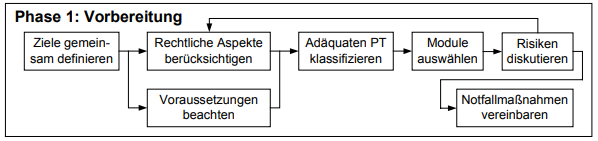
\includegraphics[width=\textwidth]{vorbereitungpt.png}
	\caption{Phase 1 – Vorbereitung des Penetrationstests}
\end{figure}


\cite[100-101]{pt03bsi}.

\subsection{Informationsbeschaffung}

\cite[102-103]{pt03bsi}.

\subsection{Bewertung der Informationen / Risikoanalyse}

\cite[103-104]{pt03bsi}.

\subsection{Aktive Eindringversuche}

\cite[104-105]{pt03bsi}.

\subsection{Abschlussanalyse / Nacharbeiten / Clean-up}

\cite[105-106]{pt03bsi}.

\section{Ablauf eines OWASP-Testmethodiks}

\section{Manuelle Penetrationstest}

\subsection{ABC}

\section{Automatisierte Penetrationstest}

\subsection{ABC}

\section{Vor- und Nachteile zwischen manuelle und automatisierte Penetrationstest}